\documentclass[10pt]{article}

% Geometry for page layout
\usepackage[utf8]{inputenc}
\usepackage[T1]{fontenc}
\usepackage[french]{babel} % Language 'english' or 'french', delete out/ if changing language
\usepackage{geometry}
\geometry{a4paper, margin=1in}

% Packages
\usepackage{amsmath}
\usepackage{graphicx}
\usepackage{subcaption}
\usepackage{fancyhdr}
\usepackage{lipsum}
\usepackage{hyperref}
\usepackage{microtype}
\usepackage{multicol}
\usepackage{csquotes}
\usepackage{listings}
\usepackage{xcolor}
\usepackage{sectsty}
\usepackage{enumitem}
\usepackage{array}
\usepackage{booktabs}
\usepackage{pdfpages}
\usepackage{indentfirst}
\usepackage{parskip}
\usepackage[scaled]{helvet}
\renewcommand{\familydefault}{\sfdefault}
\setlength{\parindent}{15pt}
\setlength{\parskip}{1em}

% Definitions
\definecolor{bleu_ece}{HTML}{00727A}
\newcommand{\bleuece}{bleu_ece}
\definecolor{bleu_google}{HTML}{1A0DAB}
\newcommand{\bleugoogle}{bleu_google}
\definecolor{orange}{HTML}{FF5733}
\newcommand{\orange}{orange}

\newcommand{\mytitle}{Projet de Fin d'Études \textit{PFE24-P-282}}
\newcommand{\myauthor}{
    Pierre LAPOLLA \and
    Matéo DOMINGUEZ \and
    Alban GAUTROT \and
    Thomas ROUSTAN \and
    Arnaud BECKER \and
    Vincent JOUANNEAU
}
% Hyperref setup
\hypersetup{
    colorlinks=true,
    linkcolor=\bleuece,
    urlcolor=\bleugoogle,
    citecolor=\orange,
    pdfborder={0 0 0}
}

% Section styles
\sectionfont{\color{\bleuece}}
\subsectionfont{\color{\bleuece}}
\subsubsectionfont{\color{\bleuece}}


% Header and footer
\fancypagestyle{plain}{
    \fancyhf{}
    \fancyhead[L]{}
    \fancyhead[C]{}
    \fancyhead[R]{
\includegraphics[height=3em]{images/logo_ece}}
    \fancyfoot[L]{\scriptsize \textit{\mytitle}}
    \fancyfoot[C]{\thepage}
    \fancyfoot[R]{\scriptsize \textit{}}
    \renewcommand{\headrulewidth}{0pt}
    \renewcommand{\footrulewidth}{0pt}
}
\pagestyle{plain}

% Title and authors, see text definition above
\title{\mytitle}
\author{\myauthor}
\date{} % \date{\today}

\begin{document}

    \maketitle

\section*{Jeu Mobile Action-RPG Basé sur les Activités Physiques}\label{sec:sujet}
\textbf
{Comment concevoir un jeu mobile action-RPG qui intègre de manière fluide les activités physiques et les données de
sommeil du joueur pour influencer le gameplay, tout en offrant une expérience de jeu captivante et motivante ? }

Les jeux vidéo mobiles connaissent une popularité croissante avec plus de 2,7 milliards de joueurs dans le monde en
2023.
Les jeux de rôle action (Action-RPG) sont particulièrement prisés pour leur gameplay dynamique et immersif.
Parallèlement, le suivi des activités physiques et des cycles de sommeil est devenu une tendance importante avec
l'adoption massive de montres connectées et d'applications de bien-être.
Associer le gameplay à la vie réelle du joueur en utilisant ses données de santé et de bien-être ouvre la voie à une
expérience ludique unique et motivante.
En intégrant l’activité physique et les données de sommeil, ce jeu pourrait proposer une progression personnalisée en
fonction des efforts réels du joueur, l’incitant à adopter un mode de vie plus sain.

\tableofcontents

\vfill
\begin{center}
    \textit{The \LaTeX{} template utilized for this document is available at:
    \url{https://github.com/PierreLapolla/tex_template.git}}
\end{center}
\newpage

    \section{Première semaine}\label{sec:semaine1}

\begin{figure}[htbp]
    \centering
    \begin{subfigure}[b]{0.45\textwidth}
        \centering
        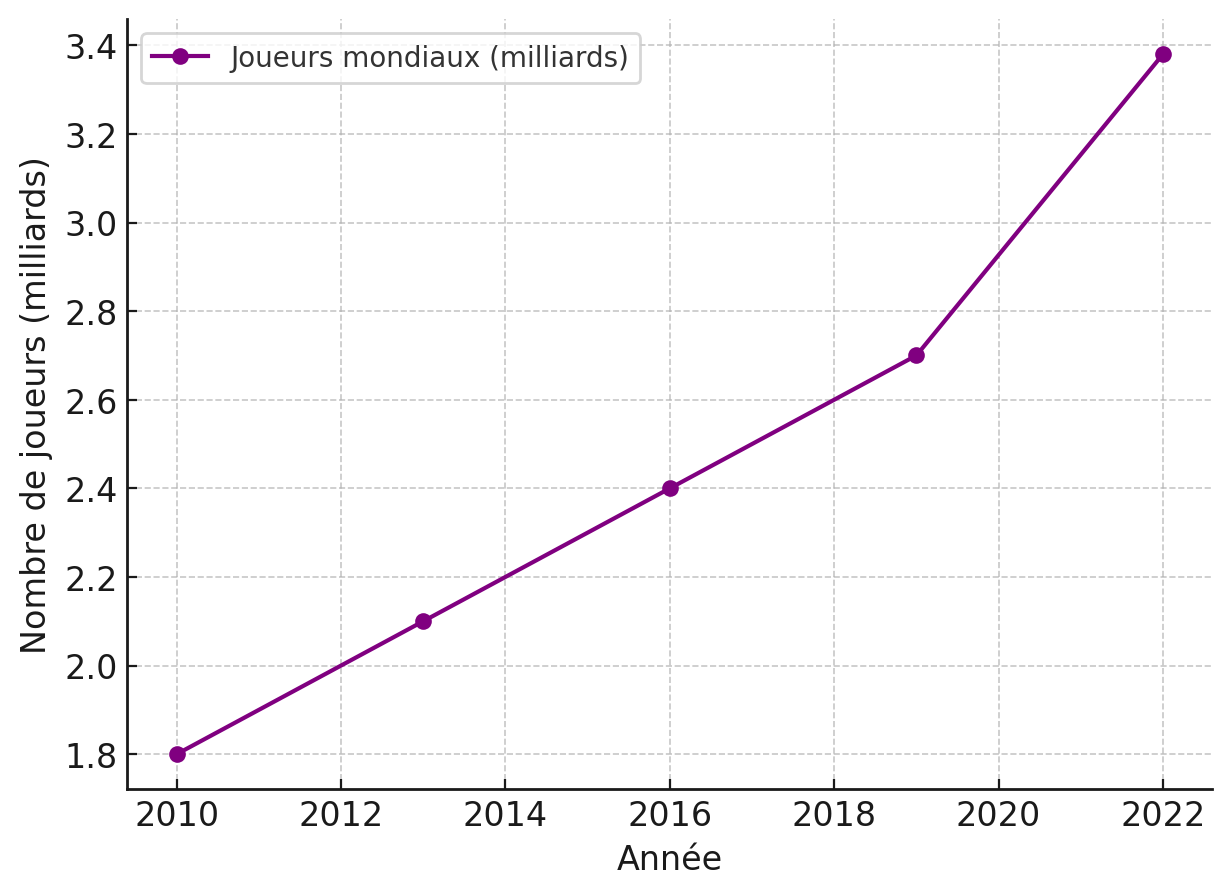
\includegraphics[width=\textwidth]{images/nombre_joueurs}
        \caption{Nombre de joueurs~\cite{newzoo_gaming_market_2023}}
        \label{fig:nombre-joueurs}
    \end{subfigure}
    \hfill
    \begin{subfigure}[b]{0.45\textwidth}
        \centering
        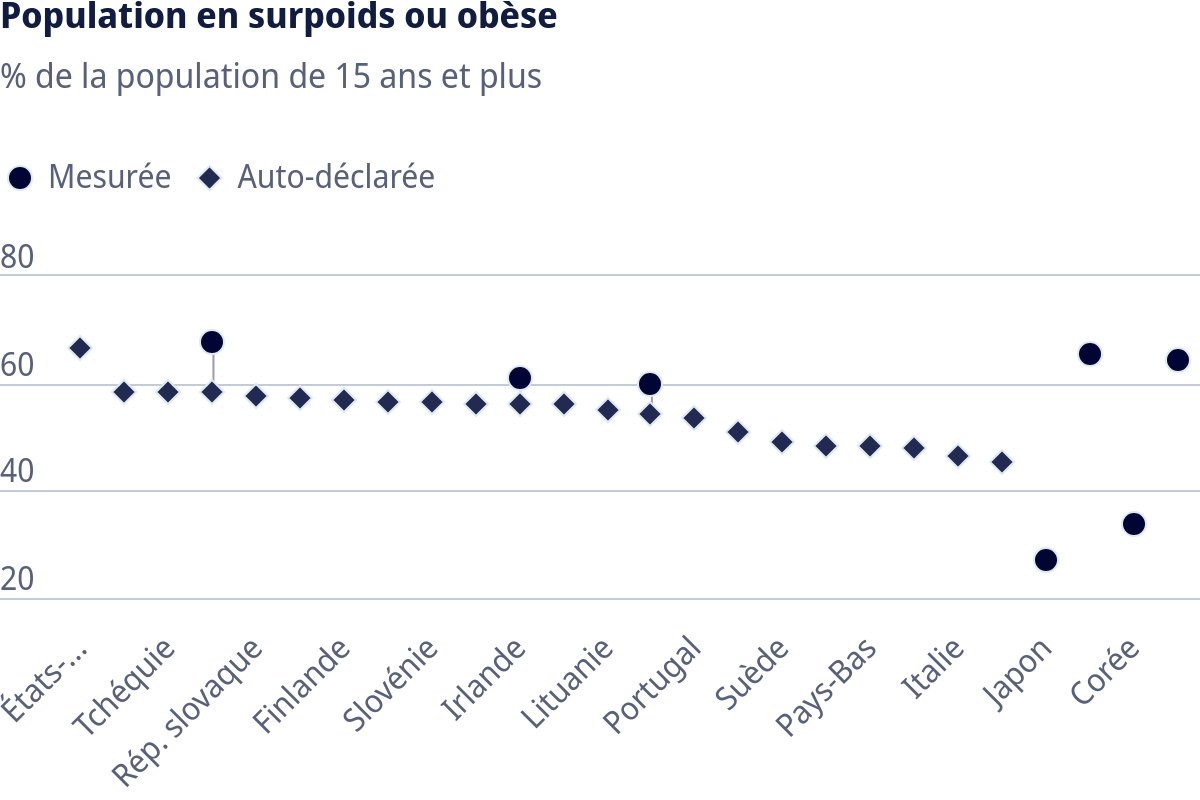
\includegraphics[width=\textwidth]{images/taux_obesite}
        \caption{Taux de \hyperref[itm:surpoids]{surpoids}~\cite{oecd_obesity_2019}}
        \label{fig:taux-obesite}
    \end{subfigure}
    \caption{Courbes des données des joueurs et du taux d'obésité.}
    \label{fig:courbes-donnees}
\end{figure}

    \section*{Glossaire}\label{sec:glossaire}

\begin{description}
    \item [Surpoids]\label{itm:surpoids}
    {
        La population en surpoids ou obèse est la part de la population ayant un poids excessif présentant des risques
        pour la santé en raison d'une proportion élevée de tissu adipeux.
        L'outil de mesure le plus fréquemment utilisé est l'indice de masse corporelle (IMC), qui évalue le poids d'un
        individu par rapport à sa taille ($\frac{\text{poids}}{\text{taille}^2}$,
        le poids étant exprimé en kilogrammes et la taille en mètres).
        Selon la classification de l'OMS, les adultes présentant un IMC compris entre 25 et 30 sont en surpoids, et ceux
        dont l'IMC est égal ou supérieur à 30 sont considérés comme obèses.
        Cet indicateur est calculé à partir de données autodéclarées (poids et taille fournis lors d'enquêtes) et de
        données mesurées (estimations précises tirées d'examens médicaux).
        Il est exprimé en pourcentage de la population âgée de 15 ans et plus.
    }
\end{description}

    \section*{Annexes}\label{sec:annexes}

    \bibliographystyle{unsrt}
    \bibliography{references}

\end{document}
